\documentclass[11pt, a4paper]{article}
\documentclass[a4paper,12pt]{report}
\usepackage[spanish]{babel}
\usepackage[utf8]{inputenc}
\usepackage{pgfplots}
\usepackage{pgfplotstable}
\pgfplotsset{compat=1.16}
\usepackage{booktabs}
\usepackage{siunitx}
\usepackage[american]{circuitikz}
\usepackage{amsmath}

\begin{document}

\part{Ejercicio 1}
\section{Introcucción}
	Se nos pidió realizar dos circuitos, el circuito derivador e integrador, que como sus nombres indican se encargan de mostrar a la salida la derivada  o integral respectivamente de su señal de entrada.
	Como se indica por consigna se utilizó el amplificador operacional LM833 y el valor comercial más cercano al pedido tanto de resistencia como de capacitor, estos son $R \ = \ 39k \Omega$ y $C \ = \ 2.7 nF$.

$R=40k\sigma -> 39k$
$C = 2.5 nF -> 2.7 nF$
\section{Cálculo de $\frac{V_{out}}{V_{in}}$}
Mientras en uno de los dos circuitos la resistencia y la impedancia tienen una disposición, para el otro se intercambian de lugar, por lo que los siguientes cálculos se realizaron con impedancias $Z_1$ y $Z_2 $ como se muestra en la Figura \ref{circconz1z2} y luego se reemplazó con el valor correspondiente al circuito al que se hizo mención.

\begin{figure}[h!]
\centering
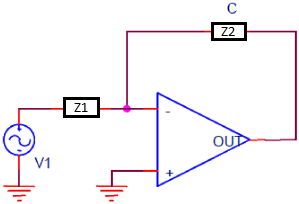
\includegraphics[scale=0.5]{circconz1z2.png}
\label{circconz1z2}
\caption{Circuito con impedancias Z1 y Z2.}
\end{figure}


\subsection{Idealidad}
\begin{equation}
	H(s) = \dfrac{V_{out}}{V_{in}} = H_{ideal} = H_I= G_{ideal} = G_I 
\end{equation}

\subsection{Con $A_{vol}$ finito}
Si dejamos de lado el caso ideal y consideramos que $A_{vol}$ no es infinita, se consigue el siguiente sistema de ecuaciones:

\begin{equation}
\begin{cases}
V_{out} = A_{vol} \ (V^+ - V^-) = - A_{vol} \ V^- \\ V_{out} - V^- = i \ Z_2 \\ V_{out} - V_{in} = i \ (Z_1+Z_2) 
\end{cases} 
\end{equation}

\begin{equation}
H(s) = - \dfrac{Z_2}{Z_1} \dfrac{1}{1+\dfrac{1+\dfrac{Z_2}{Z_1}}{A_{vol}}}
= -
\dfrac{A_{vol} \ Z_2}{Z_2 + Z_1 (A_{vol} +1)}
\end{equation}

Si $A_{vol} \longrightarrow \infty$ obtenemos la expresión para $H(s)$ vista para el caso ideal.
También podemos escribir $H(s)$ en función de $G_I$:
\begin{equation}
H(s) = \dfrac{A_{vol \ Z_2} \ G_I}{A_{vol} + 1 - G_I} 
\end{equation}

Viendo el datasheet del amplificador operacional utilizado se notó que $90 \ dB< A_{vol} < 110 \ dB$ a condiciones normales de temperatura ($25 \ ºC$) y alimentando con $\pm 15 \ V$.

\subsection{Con $A_{vol}(w)$ con polo dominante}
\begin{equation}
H(s) = - \dfrac{\dfrac{A_{vol}}{1+\dfrac{s}{w_p}} \ Z_2}{Z_2 + Z_1 \left(\dfrac{A_{vol}}{1+\dfrac{s}{w_p}} +1 \right)} 
=
-\dfrac{A_{vol} \ Z_2}{(Z_1+Z_2) \left(\dfrac{s}{w_p}+1 \right)+ A_{vol} \ Z_1}
\end{equation}

%-\frac{\mathrm{A_{vol}} \ Z_{2}}{\left(\dfrac{s}{\mathrm{w_p}}+1\right)\,\left(Z_{2}+Z_{1}\,\left(\dfrac{\mathrm{A_{vol}}}{\dfrac{s}{\mathrm{w_p}}+1}+1\right)\right)}

%= - \dfrac{Z_2 \ \left( \dfrac{A_{vol} \ w_p}{s}  + 1 \right)}{Z_2 + Z_1 \ \left( \dfrac{A_{vol} \ w_p}{s}  + 1 \right)}%
En este caso también se aplica que si $A_{vol} \longrightarrow \infty$ obtenemos la expresión para $H(s)$ vista para el caso ideal.
El datasheet nos informa que el valor de \textit{BWP}del \textit{LM833} es de $15 \ MHz$.
Si recordamos lo siguiente podemos obtener el valor de $w_p$.
\begin{equation}
BWP = A_{vol} \ . \ w_p \Rightarrow w_p= 2 \ . \pi \ \frac{BWP}{A_{vol}}= 2 \ . \ \pi \ \frac{15x10^6}{10^{\frac{110}{20}}} = 2 \ . \ \pi \ . \ 47,4342 \ Hz
\end{equation}

\section{Circuito Derivador}

\begin{figure}[h!]
\centering
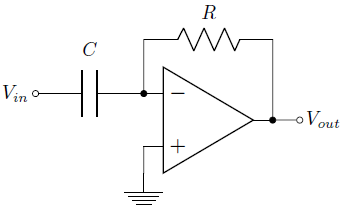
\includegraphics[scale=0.5]{circuitoderivador.png}
\label{circuitoderivador}
\caption{Circuito derivador.}
\end{figure}
En este caso $Z_1=\dfrac{1}{s \ C}$ y $Z_2= R$.

\subsection{Ganancia Ideal}

\begin{equation}
G_I=H_{ideal}(s)= - \ R \ . \ C \ . \ s
\end{equation}


\begin{center}
	\begin{figure}[h!]	
	\makebox[\textwidth]{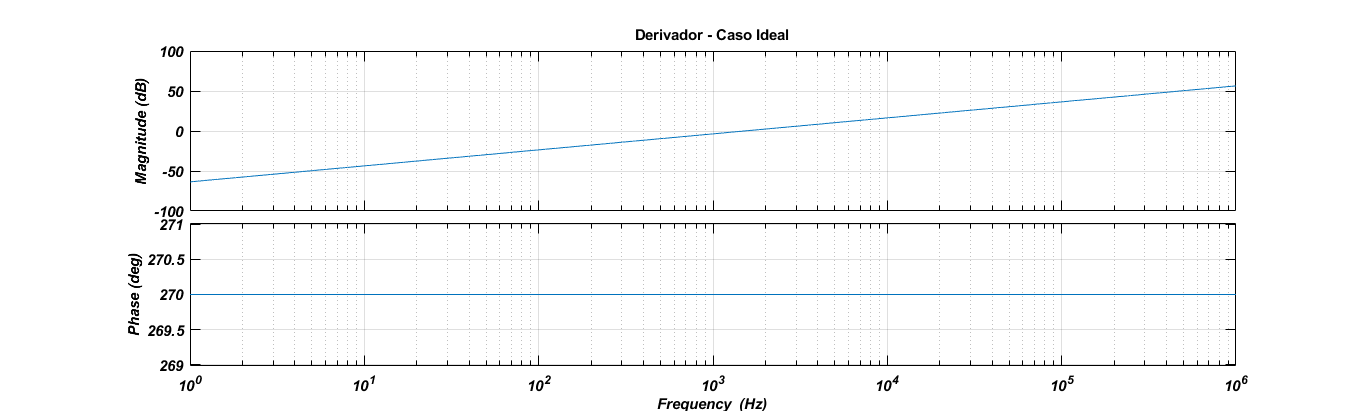
\includegraphics[width=\paperwidth]{Derivador-CasoIdeal.png}}
	\label{avolidealderivador}
	\caption{Ganancia para el caso ideal del derivador.}
	\end{figure}
\end{center}

Si realizó la antitransformada recordando que $H(s)= \dfrac{V_{out}}{V_{in}}$ obtenemos:
\begin{equation} 
v_{out} (t) = - \ R \ . \ C \ . \ \dfrac{\partial v_{in}(t)}{\partial t}
\end{equation}
Donde se observa que la función a la salida es la derivada de la función a la entrada multiplicada por una constante que es $- R C$.

\subsection{Avol finito}
\begin{equation}
H(s) = - \dfrac{A_{vol} \ . \ C \ . \ R \ . \ s}{A_{vol} + C \ . \ R \ . \ s +1 } 
= -
\left( \dfrac{A_{vol} \ . \ R \ . \ C}{A_{vol} + 1} \right) \ . \ \dfrac{s}{ \left( \dfrac{s}{\dfrac {A_{vol} +1}{R \ . \ C}} \right) + 1}
\end{equation}

Se observa que se agrega en este caso un polo en $f = \dfrac{1}{2 \ . \ \pi} \ . \ \dfrac {A_{vol} +1}{R \ . \ C} \sim 478 \ MHz $, notando así en la Figura \ref{avolfinitoderivador} que la ganancia comienza a tomar un valor constante  cerca de este valor mientras que le fase tiene un cambio de $-90$ grados lento que comienza apróximadamente a los $50 \ MHz$ y termina de caer alrededor de los $5 \ GHz$
. Mientras no se trabaje cerca de estos valores de frecuencia se puede decir que el comportamiento del circuito no se ve afectado y que se comporta como el ideal. 

\begin{figure}[h!]
	\begin{center}
		\makebox[\textwidth]{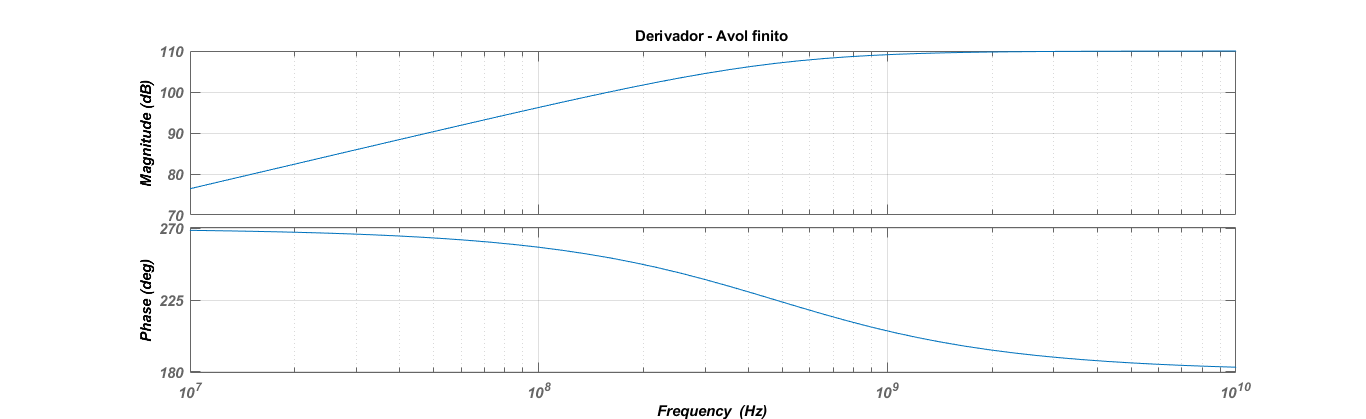
\includegraphics[width=\paperwidth]{Derivador-AvolfinitoBodeAutomatico.png}}
		\label{avolfinitoderivador}
		\caption{Ganancia para el caso con $A_{vol}$ finito del derivador.}
	\end{center}
\end{figure}

\subsection{$A{vol}(w)$ con polo dominante}

\begin{equation}
H(s) = - \left( \dfrac{A_{vol} \ . \ C \ . \ R}{A_{vol} + 1} \right) \ . \ \dfrac{s}{ \dfrac{s^2}{\dfrac{(A_{vol}+1)}{C \ . \ R}} + \dfrac{1+ C \ . \ R \ . \ w_p}{(A_{vol} + 1) \ . \ w_p} \ . \ s + 1} 
\end{equation}

En este tercer caso se observa que hay un polo de segundo orden en $f_0 = \dfrac{1}{2 \ . \pi} \sqrt{\dfrac{(A_{vol}+1)}{C \ . \ R} \ w_p} \sim 150 \ kHz$.

\begin{figure}[h!]
	\begin{center}
		\makebox[\textwidth]{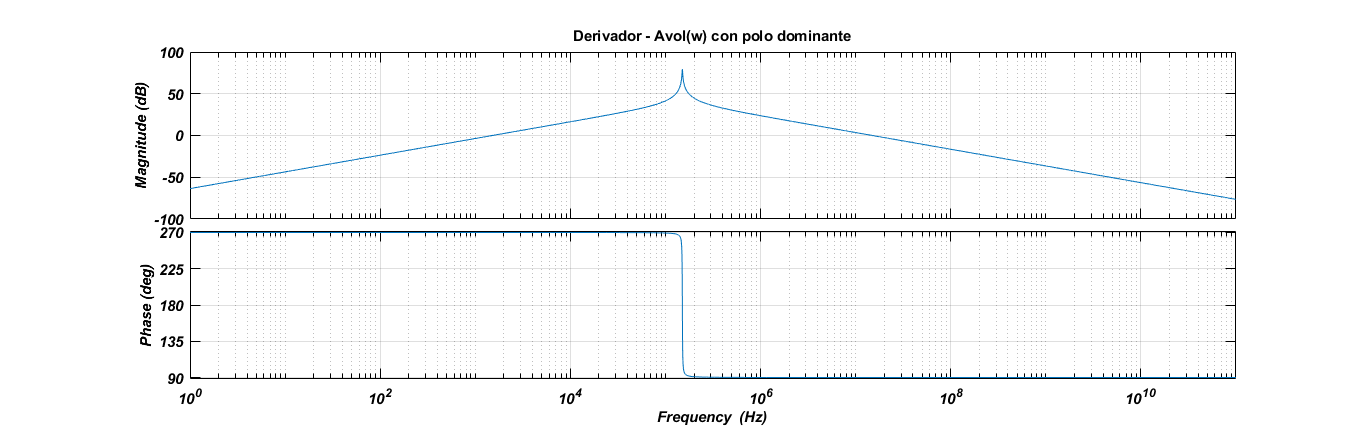
\includegraphics[width=\paperwidth]{Derivador-Avol(w)conpolodominante.png}}
		\label{avolpolodominantederivador}
		\caption{Ganancia para el caso con $A_{vol}(w)$ con polo dominante del derivador.}
	\end{center}
\end{figure}

A partir de los $100 \ kHz$ se puede notar que comienza a afectar el polo dominante como un sobrepico en la amplitud y un cambio rápido de $-180$ grados

\subsection{Comparación de los 3 casos}
\begin{figure}[h!]
	\begin{center}
		\makebox[\textwidth]{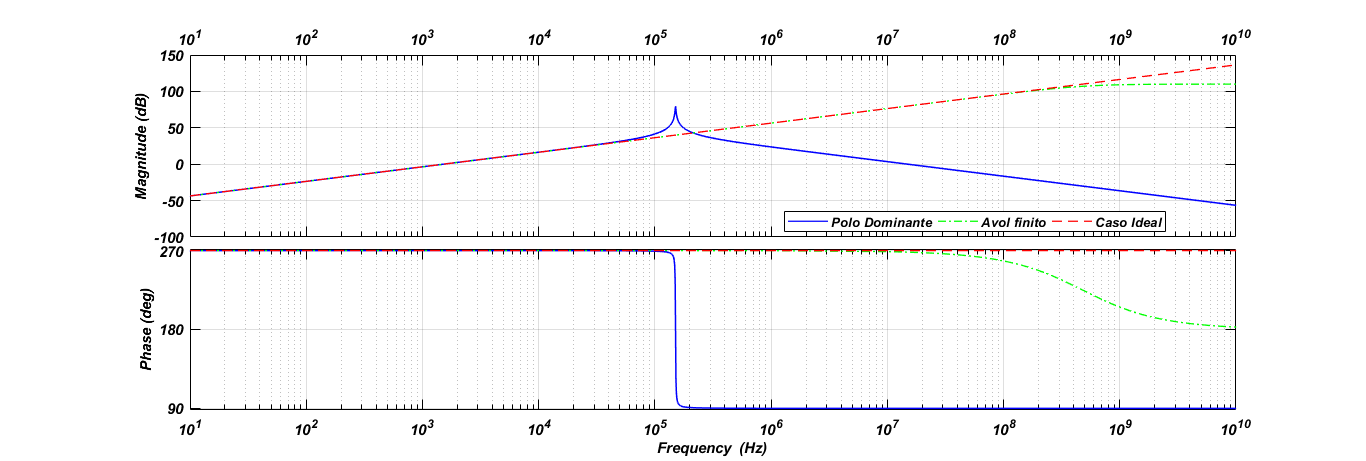
\includegraphics[width=\paperwidth]{BodesSuperpuestos.png}}
		\label{avolpolodominante}
		\caption{Superposición de los tres casos.}
	\end{center}
\end{figure}
Viendo el gráfico se notó que a frecuencias menores a aproximadamente $70 \ kHz$ tanto la amplitud como la fase de las tres funciones se comportan de forma idéntica, por lo que si trabajamos con frecuencias menores a $70 \ kHz$ el circuito debe cumplir con el propósito de su diseño, el de derivar.

\subsection{Simulación LTSpice}

\subsection{Medición}

\section{Impedancias de entrada teóricas}
\subsubsection{Primer Caso}
\begin{equation}
	Z_{in}=Z_1
\end{equation}
\subsubsection{Segundo Caso}

\subsubsection{Tercer Caso}
\section{Conclusión}

\end{document}